\section{Co-Saliency based Color Design}
Given multiple labeled scatterplots with the same class labels (or a subset thereof), each scatterplot $\mathbf{X}^j$ has $M$ classes and $n_j$ data items $\{\mathbf{x}^j_1, \cdots, \mathbf{x}^j_{n_j}\}$, where each $\mathbf{x}^j_t$ has a label
$l(\mathbf{x}^j_t)$ and the $i$-th class (with $n^j_i$ data points) consists of $\{\mathbf{x}_{i,1}^j, \cdots , \mathbf{x}_{i,n^j_i}^j\}, i \in  \{ 1, \cdots, m \} $.
All visualizations use the same  background color $\mathbf{c}_b$ and the same color mapping scheme $\tau: L \mapsto c$. Our goal is to find the best mapping $\tau$ that supports effective comparison of multiple categorical scatterplots.

In line with the design requirements of natural image comparison and categorial data visualization ~\cite{Jacobs10,Gleicher18,Lu21},
%~\cite{itti1998model,cheng2014global,zhang2018review},
our problem is formulated based on the following three design requirements:
\begin{enumerate}[label=(\roman*),nosep]
\item \textbf{DR1:} highlighting the most concerned classes between visualizations as much as possible for an efficient comparison;
\item \textbf{DR2:} maximizing the visual discrimination between classes in individual visualizations for an efficient exploration of multi-class data; and
\item \textbf{DR3:} providing flexible interactions for the exploration of relationships among the compared datasets.
%co-salient classes should follow the principles of visual salience in individual visualizations so that the co-salient classes can be easily identified.
\end{enumerate}
Although visual comparison is an essential part of interactive data analysis, most of  the existing  colorization techniques~\cite{Gramazio17, Lu21} attempt to meet DR2. The key challenge in meeting DR1 is that we need a proper model to characterize the most salient features in multiple visualizations.
To address this issue, we propose a categorical visualization co-saliency model that calculates the saliency of each data item in the context of other similar visualizations. Integrating this model into the objective of state-of-the-art color mapping selection or generation frameworks~\cite{Wang2018,Lu21}, we can
generate proper color mappings to highlight salient differences between juxtaposed categorical visualizations.

\subsection{Co-saliency for Multi-class Scatterplots }
Following the definition of image co-saliency~\cite{Jacobs10}, we model the class co-saliency with two factors: class importance between scatterplots and class contrast within scatterplots. The class importance describes how much each class should stand out from the visualizatioin. While the class contrast measures the distinctness from neighboring classes and the background, which is similar to perceptual class separability~\cite{Aupetit02,Wang2018}. Hence, we define two types of class contrasts: contrast with neighboring classes and contrast to the background.
Analogous to bottom-up image co-saliency models~\cite{Jacobs10,Fu13}, the co-saliency of the $i$th class is defined as the product between class importance and  class contrast score to emphasize the target class, and the co-saliency for $M$ classes:
\begin{equation}
% E_{CoS} = \sum_i   \sum_j (1-\lambda) \alpha^j_i  \exp(\theta_i) + \lambda \beta_i  f(\theta_i)
E_{CoS} = \sum_i    \left(\sum_j \frac{1}{n^j_i}(\lambda \alpha^j_i + (1-\lambda) \beta^j_i) \right)  \exp(\theta_i)
	\label{eq:cosaliency}
\end{equation}
where $\theta_i$ is the importance of the $i$th class, $\alpha^j_i$ is the contrast with neighboring classes of the $i$th class in the $j$th scatterplot, $\beta^j_i$  is the contrast to the background, and $\lambda$ is a weight between them.
To better support DR1, we apply an exponential function to enlarge the weight of class importance, thus makes the target class easy to get a discriminable color from the optimization process.


\noindent\textbf{Class Contrast}.
Given the $j$th scatterplot, we define the local class contrast with both point distinctness and point contrast with background~\cite{Wang2018} based on the neighbors calculated by $\alpha$-Shape~\cite{Lu21}.  For each data point $\mathbf{x}^j_t$, we define its point distinctness as:
\begin{align}\label{eq:pd}
 \gamma (\mathbf{x}^j_t)=\frac{1}{|\Omega^j_t|} \sum_{\mathbf{x}^j_p \in \Omega^j_t}  \frac{\Delta\epsilon(\tau(l(\mathbf{x}^j_t)),\tau(l(\mathbf{x}^j_p)))}{d(\mathbf{x}^j_t,\mathbf{x}^j_p)} ,
\end{align}
where $\Omega^j_t$ is set of nearest neighbors of $\mathbf{x}^j_t$, $\tau(l(\mathbf{x}^j_p))$ is the color of $\mathbf{x}^j_p$, $\Delta \epsilon$ is the CIELAB color distance~\cite{sharma2005ciede2000} and $d$ is the Euclidean distance.
For the $i$th class, its point distinctness is the sum of all points with the same class label in the scatterplot:
\begin{align}\label{eq:pdc}
 \alpha^j_i = \frac{1}{n^j_i}\sum^{n_j}_{p}\gamma(\mathbf{x}^j_p) \delta(l(\mathbf{x}^j_p),i)
\end{align}
where $\delta(l(\mathbf{x}^j_p),i)$ is one if the class label $l(\mathbf{x}^j_p)$ is $i$ and else zero.
%
%
%However, KNNG cannot reflect the contrast among classes without any overlap. For example,  in Fig.~\ref{fig:knng}(a) the contrast between the blue class and the brown classes cannot be reflected.
%To address this issue, we introduce an additional class-center based contrast cue~\cite{Fu13}.
%Suppose the center of the $i$th class in this scatterplot is $\mu^j_i$, the class contrast is:
%\begin{align}\label{eq:cc}
% \varphi^j_i =  \frac{1}{M}\sum^M_{m}\frac{\Delta\epsilon(\tau(i),\tau(m))}{||\mu^j_m -\mu^j_i ||},
%\end{align}
%which assigns large weights to nearby classes and small ones to far-away classes. The final class contrast of the $i$th class is:
%\begin{align}\label{eq:pd}
% \alpha^j_i  = \phi^j_i  + \omega \varphi^j_i,
%\end{align}
%where the weight $\omega$ is 1.0 in our experiment.
Similar to ~\cite{Wang2018}, we define non-separability as the difference value between $\mathbf{x}^j_t$ with data points belonging to the different classes and same class, thus the contrast to the background can be defined as:
\begin{align}\label{eq:ctb}
 \rho (\mathbf{x}^j_t)=\frac{1}{|\Omega^j_t|} \sum_{\mathbf{x}^j_p \in \Omega^j_t}  \frac{(1-2\delta(l(\mathbf{x}^j_t),l(\mathbf{x}^j_p)))\Delta\epsilon(\tau(l(\mathbf{x}^j_t)),\mathbf{c}_b)}{d(\mathbf{x}^j_t,\mathbf{x}^j_p)} ,
\end{align}
the contrast to the background of the $i$th class is defined as follows:
\begin{align}\label{eq:ctbc}
 \beta^j_i = \frac{f(\theta_i)}{n^j_i}\sum^{n_j}_{p} \exp(\rho(\mathbf{x}^j_p)) \delta(l(\mathbf{x}^j_p),i)
\end{align}
where we use a piecewise function to weight the background contrast:
\begin{align}
f(\theta_i) =  \left\{ \begin{array}{ll}
1 & \textrm{if $\theta_i>\kappa$}\\
-1 & \textrm{else}
\end{array} \right.
\label{eq:piecewiseFunc}
\end{align}
$\kappa$ is a user-specified threshold with the default zero. The reason for the two different weighting schemes is that classes with less or no importance might be treated as the background by viewers~\cite{zhang2018review}. To suppress the saliency of such classes, we introduce a negative importance for them. Since $\rho (\mathbf{x}^j_t)$ might be a negative value, we apply an exponential function to transfer it to positive.

\vspace{1.5mm}
\noindent\textbf{Class Importance}.
Class importance reflects whether a class should be highlight or not. It can be specified by user or by some measures. In our paper, we use class change degree to represent the importance of each class as default.
\begin{wrapfigure}{r}{0.28\columnwidth}
	\vspace{-5mm}
	\centering
	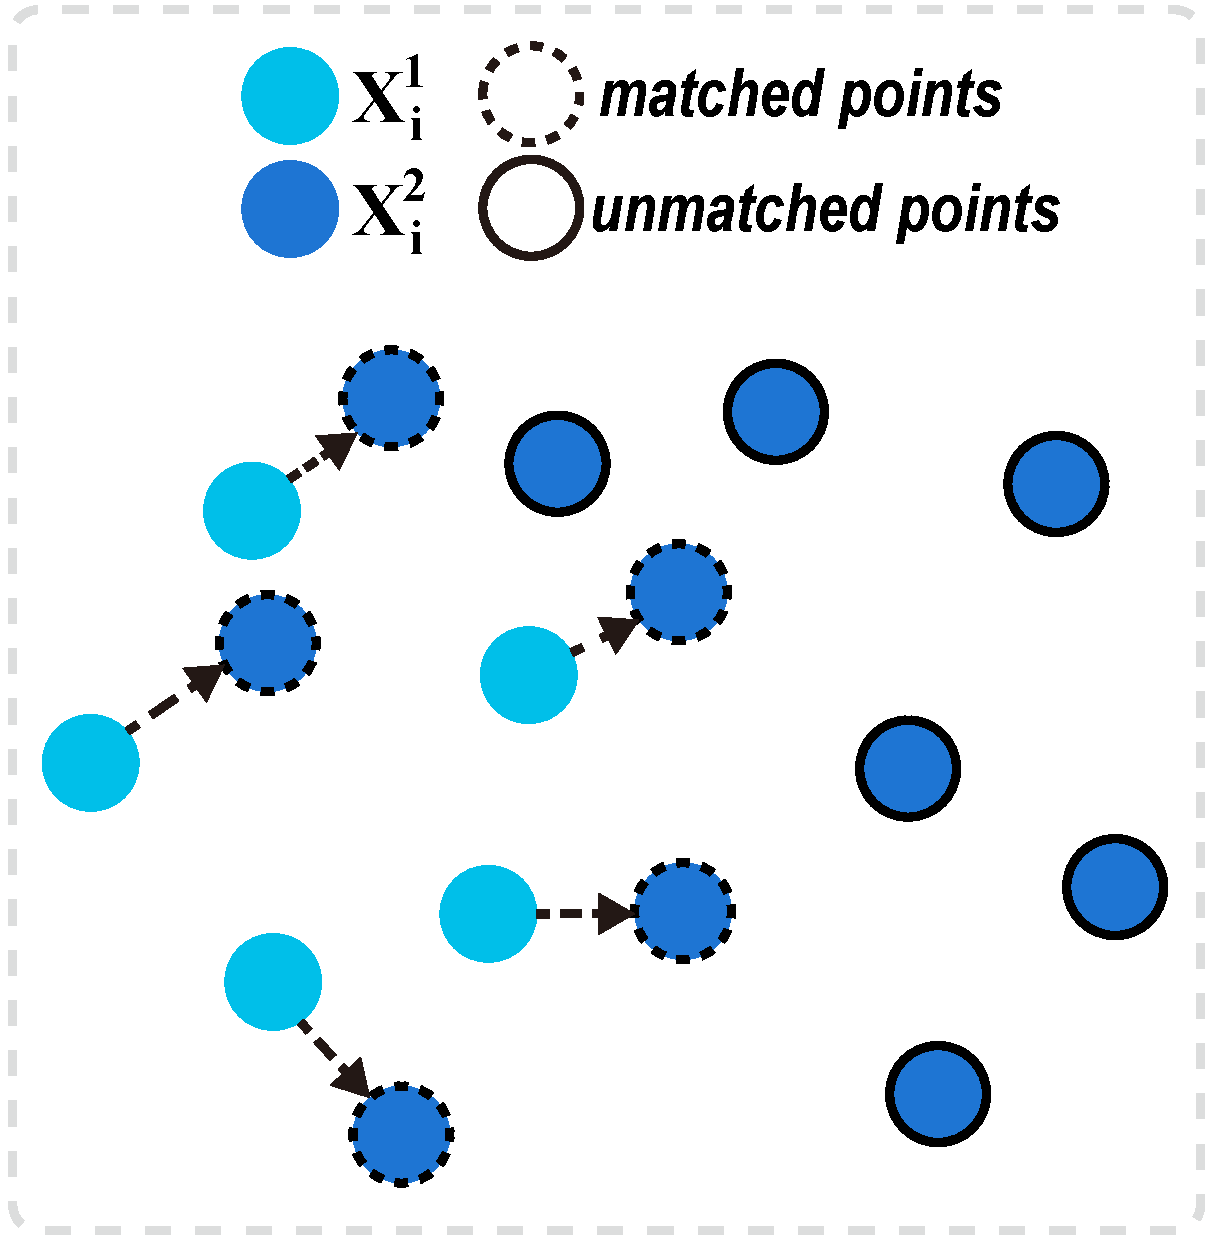
\includegraphics[width=0.28\columnwidth]{class-change-degree}
	\vspace*{-8mm}
	\caption{An one-to-one mapping for computing the changes between two classes.}
	\vspace*{-2mm}
	\label{fig:class-change-degree}
\end{wrapfigure}
To quantify how users perceive class structure changes, we measure the difference between class distributions in two scatterplots with the Earth Mover's Distance (EMD)~\cite{rubner2000earth}, a perceptual metric.
Suppose the $i$th  class with two sets of points $\mathbf{X}^1_i = \{\mathbf{x}_{i,1}^1, \cdots , \mathbf{x}_{i,n^1_i}^1\}$ and $\mathbf{X}^2_i = \{\mathbf{x}_{i,1}^2, \cdots , \mathbf{x}_{i,n^2_i}^2\}$.
Taking the Euclidian distance between two points as the cost, we need to  minimize the total matching cost
\begin{align}\label{eq:emd}
 H(\mathbf{X}^1_i, \mathbf{X}^2_i)  = \min_\chi \sum_t d(\mathbf{x}_{i,t}^1, \mathbf{x}_{i,\chi(t)}^2),
\end{align}
which constrains an one-to-one mapping $\chi$ between points (see an illustration in Fig.~\ref{fig:class-change-degree}). This is the classic bipartite matching problem, which can be solved by the Hungarian method~\cite{kuhn1955hungarian}.
When the number of points of two sets is not equal, we further take the difference between the number of points into account. In doing so, the class change degree is defined as:
\begin{align}\label{eq:cm}
 \theta_i= \frac{H(\mathbf{X}^1_i, \mathbf{X}^2_i) }{\min\{n^1_i, n^2_i\}} + \nu \frac{||n^1_i- n^2_i||}{\max\{n^1_i, n^2_i\}}
\end{align}
where both terms range within [0,1] and $\nu$ is 1.0 as the default.


